% Options for packages loaded elsewhere
\PassOptionsToPackage{unicode}{hyperref}
\PassOptionsToPackage{hyphens}{url}
\PassOptionsToPackage{dvipsnames,svgnames,x11names}{xcolor}
%
\documentclass[
  letterpaper,
  DIV=11,
  numbers=noendperiod]{scrartcl}

\usepackage{amsmath,amssymb}
\usepackage{iftex}
\ifPDFTeX
  \usepackage[T1]{fontenc}
  \usepackage[utf8]{inputenc}
  \usepackage{textcomp} % provide euro and other symbols
\else % if luatex or xetex
  \usepackage{unicode-math}
  \defaultfontfeatures{Scale=MatchLowercase}
  \defaultfontfeatures[\rmfamily]{Ligatures=TeX,Scale=1}
\fi
\usepackage{lmodern}
\ifPDFTeX\else  
    % xetex/luatex font selection
\fi
% Use upquote if available, for straight quotes in verbatim environments
\IfFileExists{upquote.sty}{\usepackage{upquote}}{}
\IfFileExists{microtype.sty}{% use microtype if available
  \usepackage[]{microtype}
  \UseMicrotypeSet[protrusion]{basicmath} % disable protrusion for tt fonts
}{}
\makeatletter
\@ifundefined{KOMAClassName}{% if non-KOMA class
  \IfFileExists{parskip.sty}{%
    \usepackage{parskip}
  }{% else
    \setlength{\parindent}{0pt}
    \setlength{\parskip}{6pt plus 2pt minus 1pt}}
}{% if KOMA class
  \KOMAoptions{parskip=half}}
\makeatother
\usepackage{xcolor}
\setlength{\emergencystretch}{3em} % prevent overfull lines
\setcounter{secnumdepth}{5}
% Make \paragraph and \subparagraph free-standing
\ifx\paragraph\undefined\else
  \let\oldparagraph\paragraph
  \renewcommand{\paragraph}[1]{\oldparagraph{#1}\mbox{}}
\fi
\ifx\subparagraph\undefined\else
  \let\oldsubparagraph\subparagraph
  \renewcommand{\subparagraph}[1]{\oldsubparagraph{#1}\mbox{}}
\fi


\providecommand{\tightlist}{%
  \setlength{\itemsep}{0pt}\setlength{\parskip}{0pt}}\usepackage{longtable,booktabs,array}
\usepackage{calc} % for calculating minipage widths
% Correct order of tables after \paragraph or \subparagraph
\usepackage{etoolbox}
\makeatletter
\patchcmd\longtable{\par}{\if@noskipsec\mbox{}\fi\par}{}{}
\makeatother
% Allow footnotes in longtable head/foot
\IfFileExists{footnotehyper.sty}{\usepackage{footnotehyper}}{\usepackage{footnote}}
\makesavenoteenv{longtable}
\usepackage{graphicx}
\makeatletter
\def\maxwidth{\ifdim\Gin@nat@width>\linewidth\linewidth\else\Gin@nat@width\fi}
\def\maxheight{\ifdim\Gin@nat@height>\textheight\textheight\else\Gin@nat@height\fi}
\makeatother
% Scale images if necessary, so that they will not overflow the page
% margins by default, and it is still possible to overwrite the defaults
% using explicit options in \includegraphics[width, height, ...]{}
\setkeys{Gin}{width=\maxwidth,height=\maxheight,keepaspectratio}
% Set default figure placement to htbp
\makeatletter
\def\fps@figure{htbp}
\makeatother

\KOMAoption{captions}{tableheading}
\makeatletter
\@ifpackageloaded{tcolorbox}{}{\usepackage[skins,breakable]{tcolorbox}}
\@ifpackageloaded{fontawesome5}{}{\usepackage{fontawesome5}}
\definecolor{quarto-callout-color}{HTML}{909090}
\definecolor{quarto-callout-note-color}{HTML}{0758E5}
\definecolor{quarto-callout-important-color}{HTML}{CC1914}
\definecolor{quarto-callout-warning-color}{HTML}{EB9113}
\definecolor{quarto-callout-tip-color}{HTML}{00A047}
\definecolor{quarto-callout-caution-color}{HTML}{FC5300}
\definecolor{quarto-callout-color-frame}{HTML}{acacac}
\definecolor{quarto-callout-note-color-frame}{HTML}{4582ec}
\definecolor{quarto-callout-important-color-frame}{HTML}{d9534f}
\definecolor{quarto-callout-warning-color-frame}{HTML}{f0ad4e}
\definecolor{quarto-callout-tip-color-frame}{HTML}{02b875}
\definecolor{quarto-callout-caution-color-frame}{HTML}{fd7e14}
\makeatother
\makeatletter
\makeatother
\makeatletter
\makeatother
\makeatletter
\@ifpackageloaded{caption}{}{\usepackage{caption}}
\AtBeginDocument{%
\ifdefined\contentsname
  \renewcommand*\contentsname{Table of contents}
\else
  \newcommand\contentsname{Table of contents}
\fi
\ifdefined\listfigurename
  \renewcommand*\listfigurename{List of Figures}
\else
  \newcommand\listfigurename{List of Figures}
\fi
\ifdefined\listtablename
  \renewcommand*\listtablename{List of Tables}
\else
  \newcommand\listtablename{List of Tables}
\fi
\ifdefined\figurename
  \renewcommand*\figurename{Figure}
\else
  \newcommand\figurename{Figure}
\fi
\ifdefined\tablename
  \renewcommand*\tablename{Table}
\else
  \newcommand\tablename{Table}
\fi
}
\@ifpackageloaded{float}{}{\usepackage{float}}
\floatstyle{ruled}
\@ifundefined{c@chapter}{\newfloat{codelisting}{h}{lop}}{\newfloat{codelisting}{h}{lop}[chapter]}
\floatname{codelisting}{Listing}
\newcommand*\listoflistings{\listof{codelisting}{List of Listings}}
\makeatother
\makeatletter
\@ifpackageloaded{caption}{}{\usepackage{caption}}
\@ifpackageloaded{subcaption}{}{\usepackage{subcaption}}
\makeatother
\makeatletter
\@ifpackageloaded{tcolorbox}{}{\usepackage[skins,breakable]{tcolorbox}}
\makeatother
\makeatletter
\@ifundefined{shadecolor}{\definecolor{shadecolor}{rgb}{.97, .97, .97}}
\makeatother
\makeatletter
\makeatother
\makeatletter
\makeatother
\ifLuaTeX
  \usepackage{selnolig}  % disable illegal ligatures
\fi
\IfFileExists{bookmark.sty}{\usepackage{bookmark}}{\usepackage{hyperref}}
\IfFileExists{xurl.sty}{\usepackage{xurl}}{} % add URL line breaks if available
\urlstyle{same} % disable monospaced font for URLs
\hypersetup{
  pdftitle={My document},
  colorlinks=true,
  linkcolor={blue},
  filecolor={Maroon},
  citecolor={Blue},
  urlcolor={Blue},
  pdfcreator={LaTeX via pandoc}}

\title{My document}
\author{}
\date{}

\begin{document}
\maketitle
\ifdefined\Shaded\renewenvironment{Shaded}{\begin{tcolorbox}[boxrule=0pt, enhanced, frame hidden, interior hidden, sharp corners, breakable, borderline west={3pt}{0pt}{shadecolor}]}{\end{tcolorbox}}\fi

\renewcommand*\contentsname{Table of contents}
{
\hypersetup{linkcolor=}
\setcounter{tocdepth}{3}
\tableofcontents
}
\hypertarget{microinjections}{%
\section*{Microinjections}\label{microinjections}}
\addcontentsline{toc}{section}{Microinjections}

\begin{tcolorbox}[enhanced jigsaw, breakable, colback=white, opacityback=0, arc=.35mm, colframe=quarto-callout-tip-color-frame, rightrule=.15mm, bottomrule=.15mm, toprule=.15mm, left=2mm, leftrule=.75mm]

\textbf{Ingredients}\vspace{2mm}

\begin{itemize}
\tightlist
\item
  3-AT sea water
\item
  PS-coated petri dish
\item
  Pipette and tips
\item
  Dejellied eggs
\item
  Sperm
\item
  Microinjection needle
\item
  Injection solution
\end{itemize}

\end{tcolorbox}

\hypertarget{preparation-of-injection-solution-and-needle}{%
\subsection{Preparation of injection solution and
needle}\label{preparation-of-injection-solution-and-needle}}

Prepare the following injection solution, preferably the same day it is
going to be used.

\begin{longtable}[]{@{}
  >{\raggedright\arraybackslash}p{(\columnwidth - 4\tabcolsep) * \real{0.2500}}
  >{\centering\arraybackslash}p{(\columnwidth - 4\tabcolsep) * \real{0.3125}}
  >{\raggedleft\arraybackslash}p{(\columnwidth - 4\tabcolsep) * \real{0.4375}}@{}}
\toprule\noalign{}
\begin{minipage}[b]{\linewidth}\raggedright
Ingradient
\end{minipage} & \begin{minipage}[b]{\linewidth}\centering
Final Quantity in 20 ul
\end{minipage} & \begin{minipage}[b]{\linewidth}\raggedleft
Volume to be added
\end{minipage} \\
\midrule\noalign{}
\endhead
\bottomrule\noalign{}
\endlastfoot
Linearised construct & 100ng & Depends on construct concentration \\
gDNA & 500ng & Depends on construct concentration \\
KCl (1M) & 0.12M & 2.4 ul \\
Glycerol (50\%) & 20\% & 8 ul \\
Control dye (10\%) & 0.25\% & 0.5 ul \\
ddH2O & - & To add up to 20 ul \\
\end{longtable}

\begin{tcolorbox}[enhanced jigsaw, breakable, colback=white, opacityback=0, arc=.35mm, colframe=quarto-callout-tip-color-frame, rightrule=.15mm, bottomrule=.15mm, toprule=.15mm, left=2mm, leftrule=.75mm]

\textbf{Linearised construct}\vspace{2mm}

This is restriction enzyme digested plasmid. For Anpep\_1, digest with
KpnI. Confirm digestion product with gel electrophoresis and use the PCR
purification kit to remove restriction enzyme from the DNA solution.

\end{tcolorbox}

\begin{tcolorbox}[enhanced jigsaw, breakable, colback=white, opacityback=0, arc=.35mm, colframe=quarto-callout-tip-color-frame, rightrule=.15mm, bottomrule=.15mm, toprule=.15mm, left=2mm, leftrule=.75mm]

\textbf{gDNA}\vspace{2mm}

HindIII digested (overnight) and purified genomic DNA extracted from
urchin epidermal tissue.

\end{tcolorbox}

\begin{tcolorbox}[enhanced jigsaw, breakable, colback=white, opacityback=0, arc=.35mm, colframe=quarto-callout-tip-color-frame, rightrule=.15mm, bottomrule=.15mm, toprule=.15mm, left=2mm, leftrule=.75mm]

\textbf{Control dye}\vspace{2mm}

Texas Red dye diluted to 10\%.

\end{tcolorbox}

Injection solution should be centrifuged for 15 minutes at max speed
immediately before filling the microinjection needle.

\hypertarget{preparation-of-the-needle}{%
\subsubsection{Preparation of the
needle}\label{preparation-of-the-needle}}

\begin{tcolorbox}[enhanced jigsaw, breakable, rightrule=.15mm, colbacktitle=quarto-callout-warning-color!10!white, leftrule=.75mm, arc=.35mm, colback=white, title=\textcolor{quarto-callout-warning-color}{\faExclamationTriangle}\hspace{0.5em}{Warning}, coltitle=black, bottomtitle=1mm, opacityback=0, titlerule=0mm, colframe=quarto-callout-warning-color-frame, toptitle=1mm, opacitybacktitle=0.6, toprule=.15mm, left=2mm, bottomrule=.15mm]

Be careful never to touch either ends of the needle!

\end{tcolorbox}

We used a Narishige puller, model PP-830

\begin{figure}

\begin{minipage}[t]{0.50\linewidth}

{\centering 

\raisebox{-\height}{

\includegraphics{micro_photos/included/needle_puller.jpg}

}

}

\subcaption{\label{fig-puller1}Needle puller machine}
\end{minipage}%
%
\begin{minipage}[t]{0.50\linewidth}

{\centering 

\raisebox{-\height}{

\includegraphics{micro_photos/included/needle_puller2.jpg}

}

}

\subcaption{\label{fig-puller2}6th grid setting}
\end{minipage}%

\caption{\label{fig-eggs}Needle puller set up}

\end{figure}

with the following settings:

Two stage: 67.4°C, 80.2°C.

Weight: 248.01 g

\begin{figure}

\begin{minipage}[t]{0.50\linewidth}

{\centering 

\raisebox{-\height}{

\includegraphics{micro_photos/included/needle_puller_weights.jpg}

}

}

\subcaption{\label{fig-weights1}Puller weights on scale}
\end{minipage}%
%
\begin{minipage}[t]{0.50\linewidth}

{\centering 

\raisebox{-\height}{

\includegraphics{micro_photos/included/puller_weight.jpg}

}

}

\subcaption{\label{fig-weights2}Puller weights on the machine}
\end{minipage}%

\caption{\label{fig-eggs}Weights used for the puller}

\end{figure}

\begin{figure}

\begin{minipage}[t]{0.50\linewidth}

{\centering 

\raisebox{-\height}{

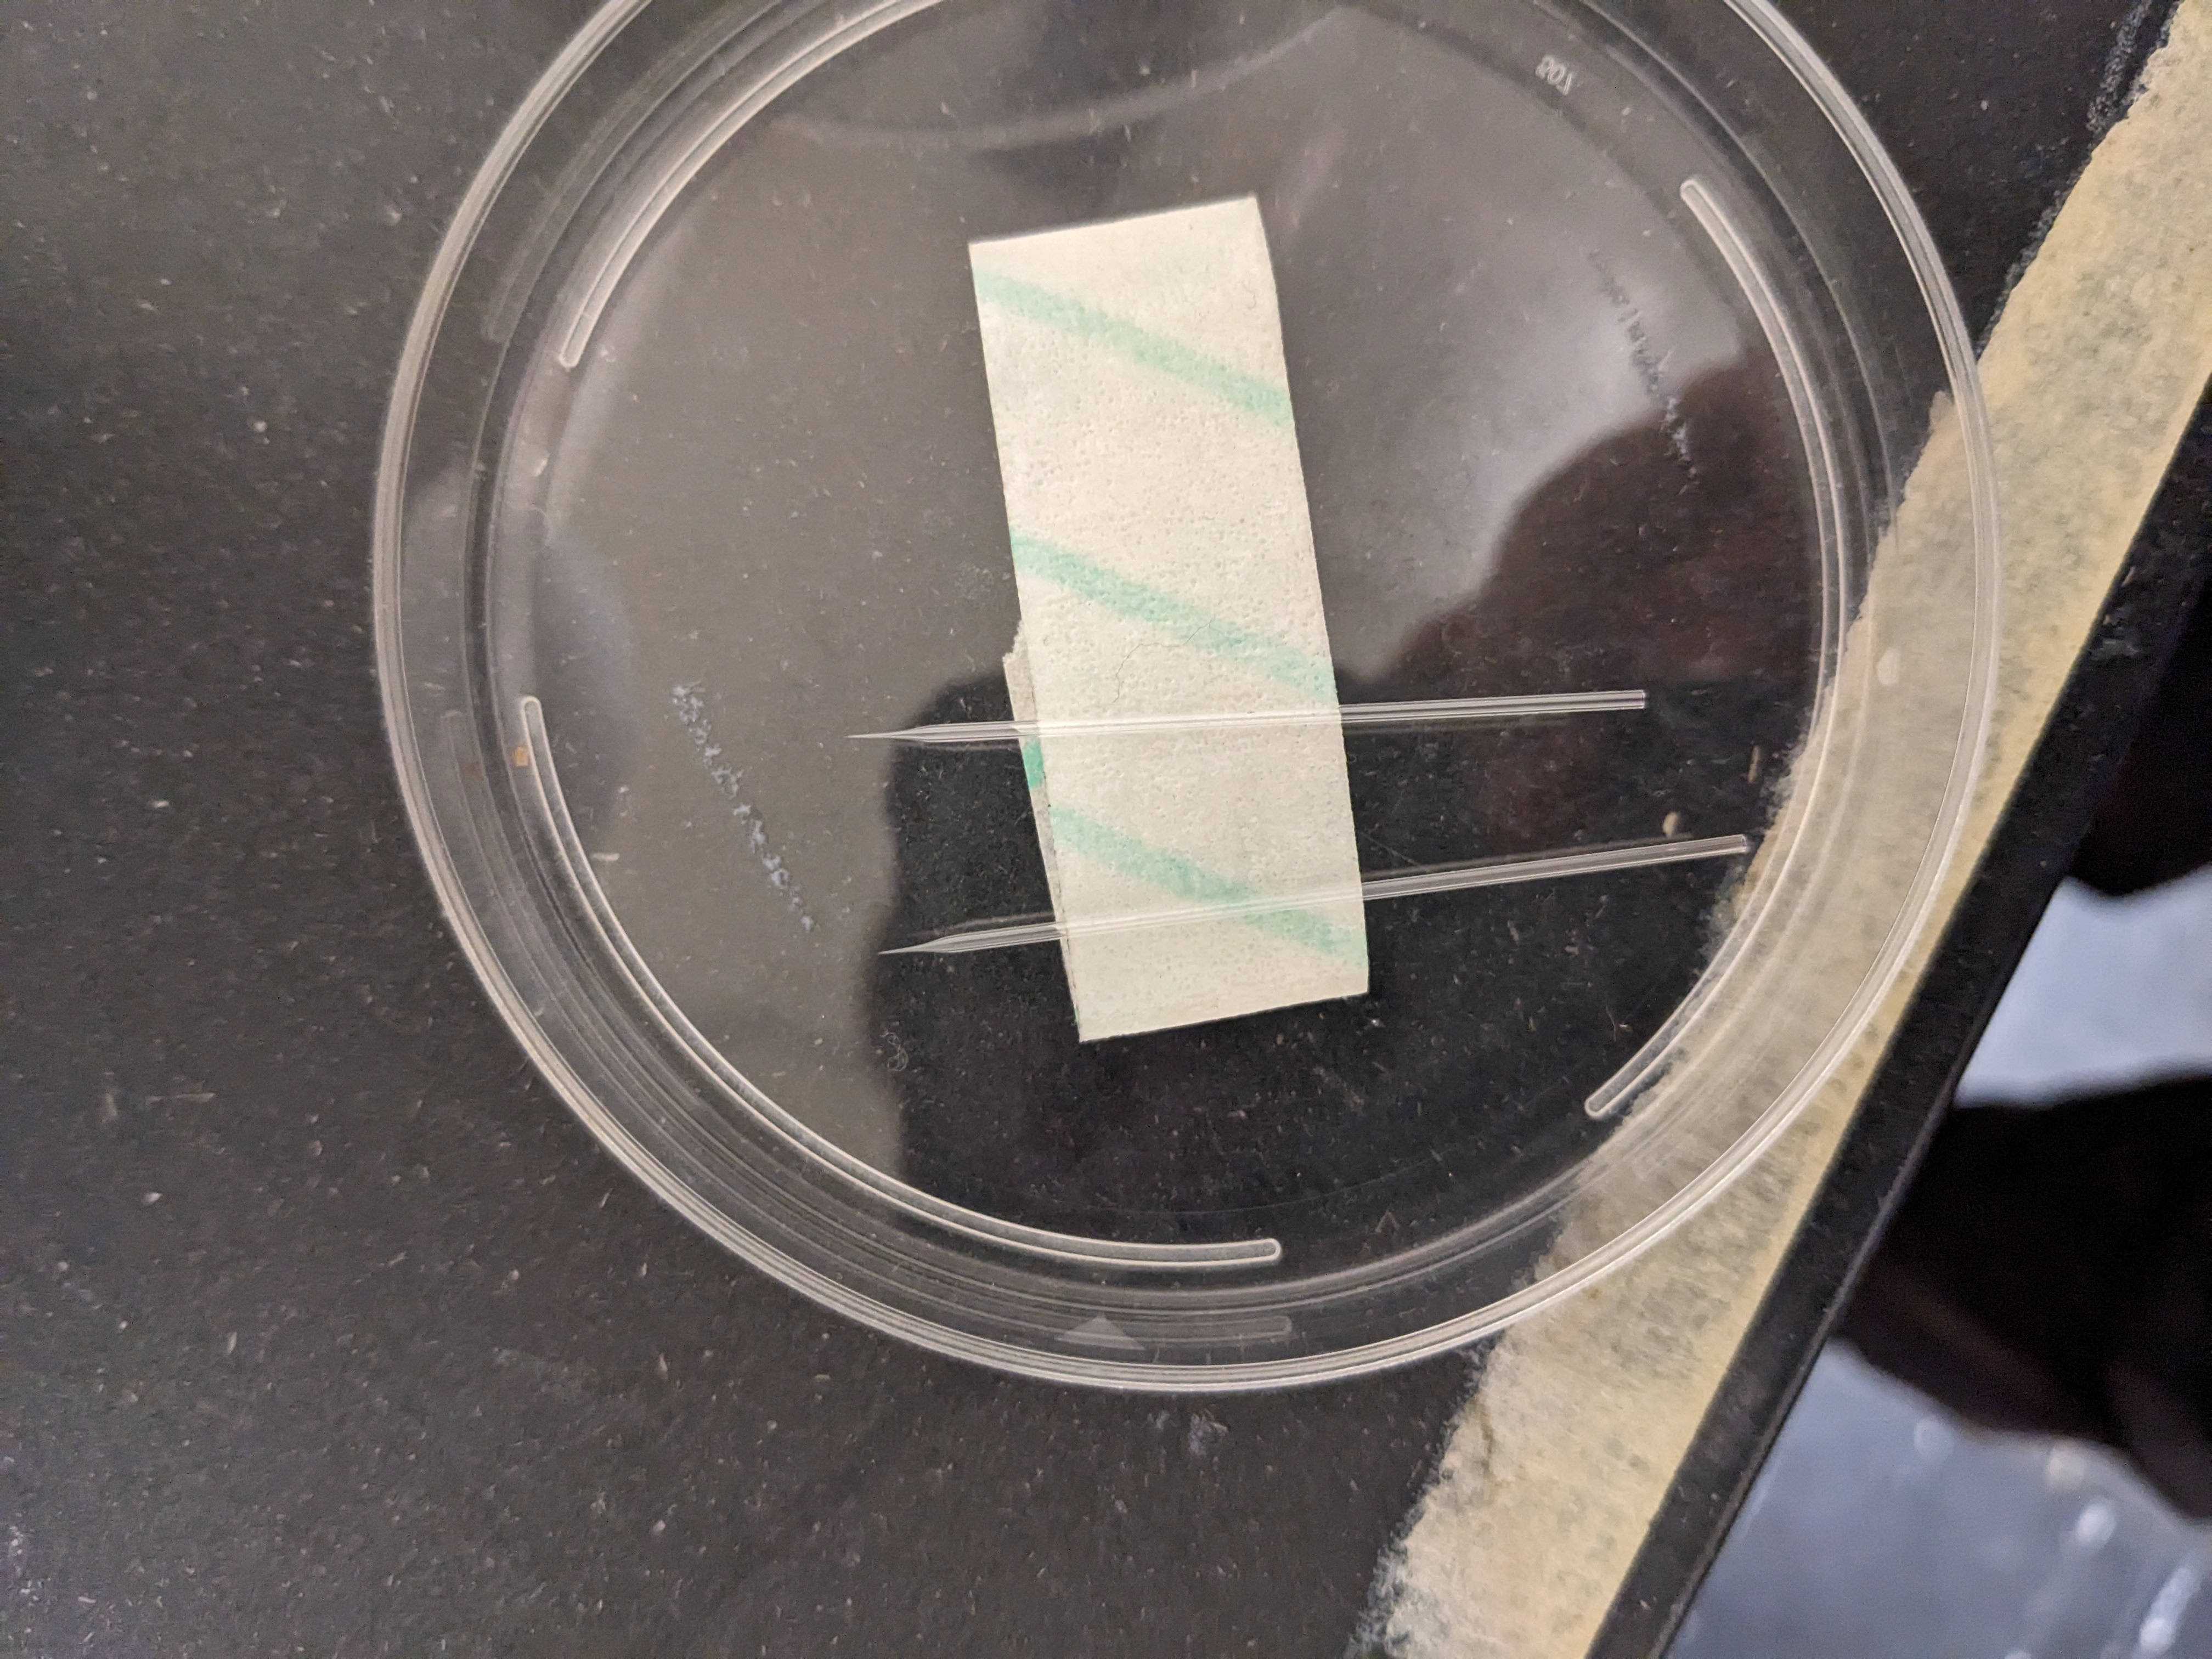
\includegraphics{micro_photos/included/needle_ends2.jpg}

}

}

\subcaption{\label{fig-doneneedles1}Storing pulled needles}
\end{minipage}%
%
\begin{minipage}[t]{0.50\linewidth}

{\centering 

\raisebox{-\height}{

\includegraphics{micro_photos/included/needles_ends.jpg}

}

}

\subcaption{\label{fig-doneneedles2}Pulled needle ends}
\end{minipage}%

\caption{\label{fig-eggs}Pulled needles}

\end{figure}

\hypertarget{filling-the-needle}{%
\subsubsection{Filling the needle}\label{filling-the-needle}}

To fill the needles, pipette up 0.5 ul of injection solution. Use a 10ul
pipette tip. Make sure to get the liquid from the top/middle of the tube
in order to avoid any precipitate stuck to the bottom/sides of the tube
during the centrifugation.

Put a piece of clay on the side of a table and push the needle upside
down into it. Fill needle by touching the end of the needle with the tip
of the pipette and pushing out the liquid with the pipette. Make sure
that the liquid enters the needle instead of just sitting on top. Wait a
few minutes for the solution to reach the bottom of the needle.

\begin{figure}

{\centering 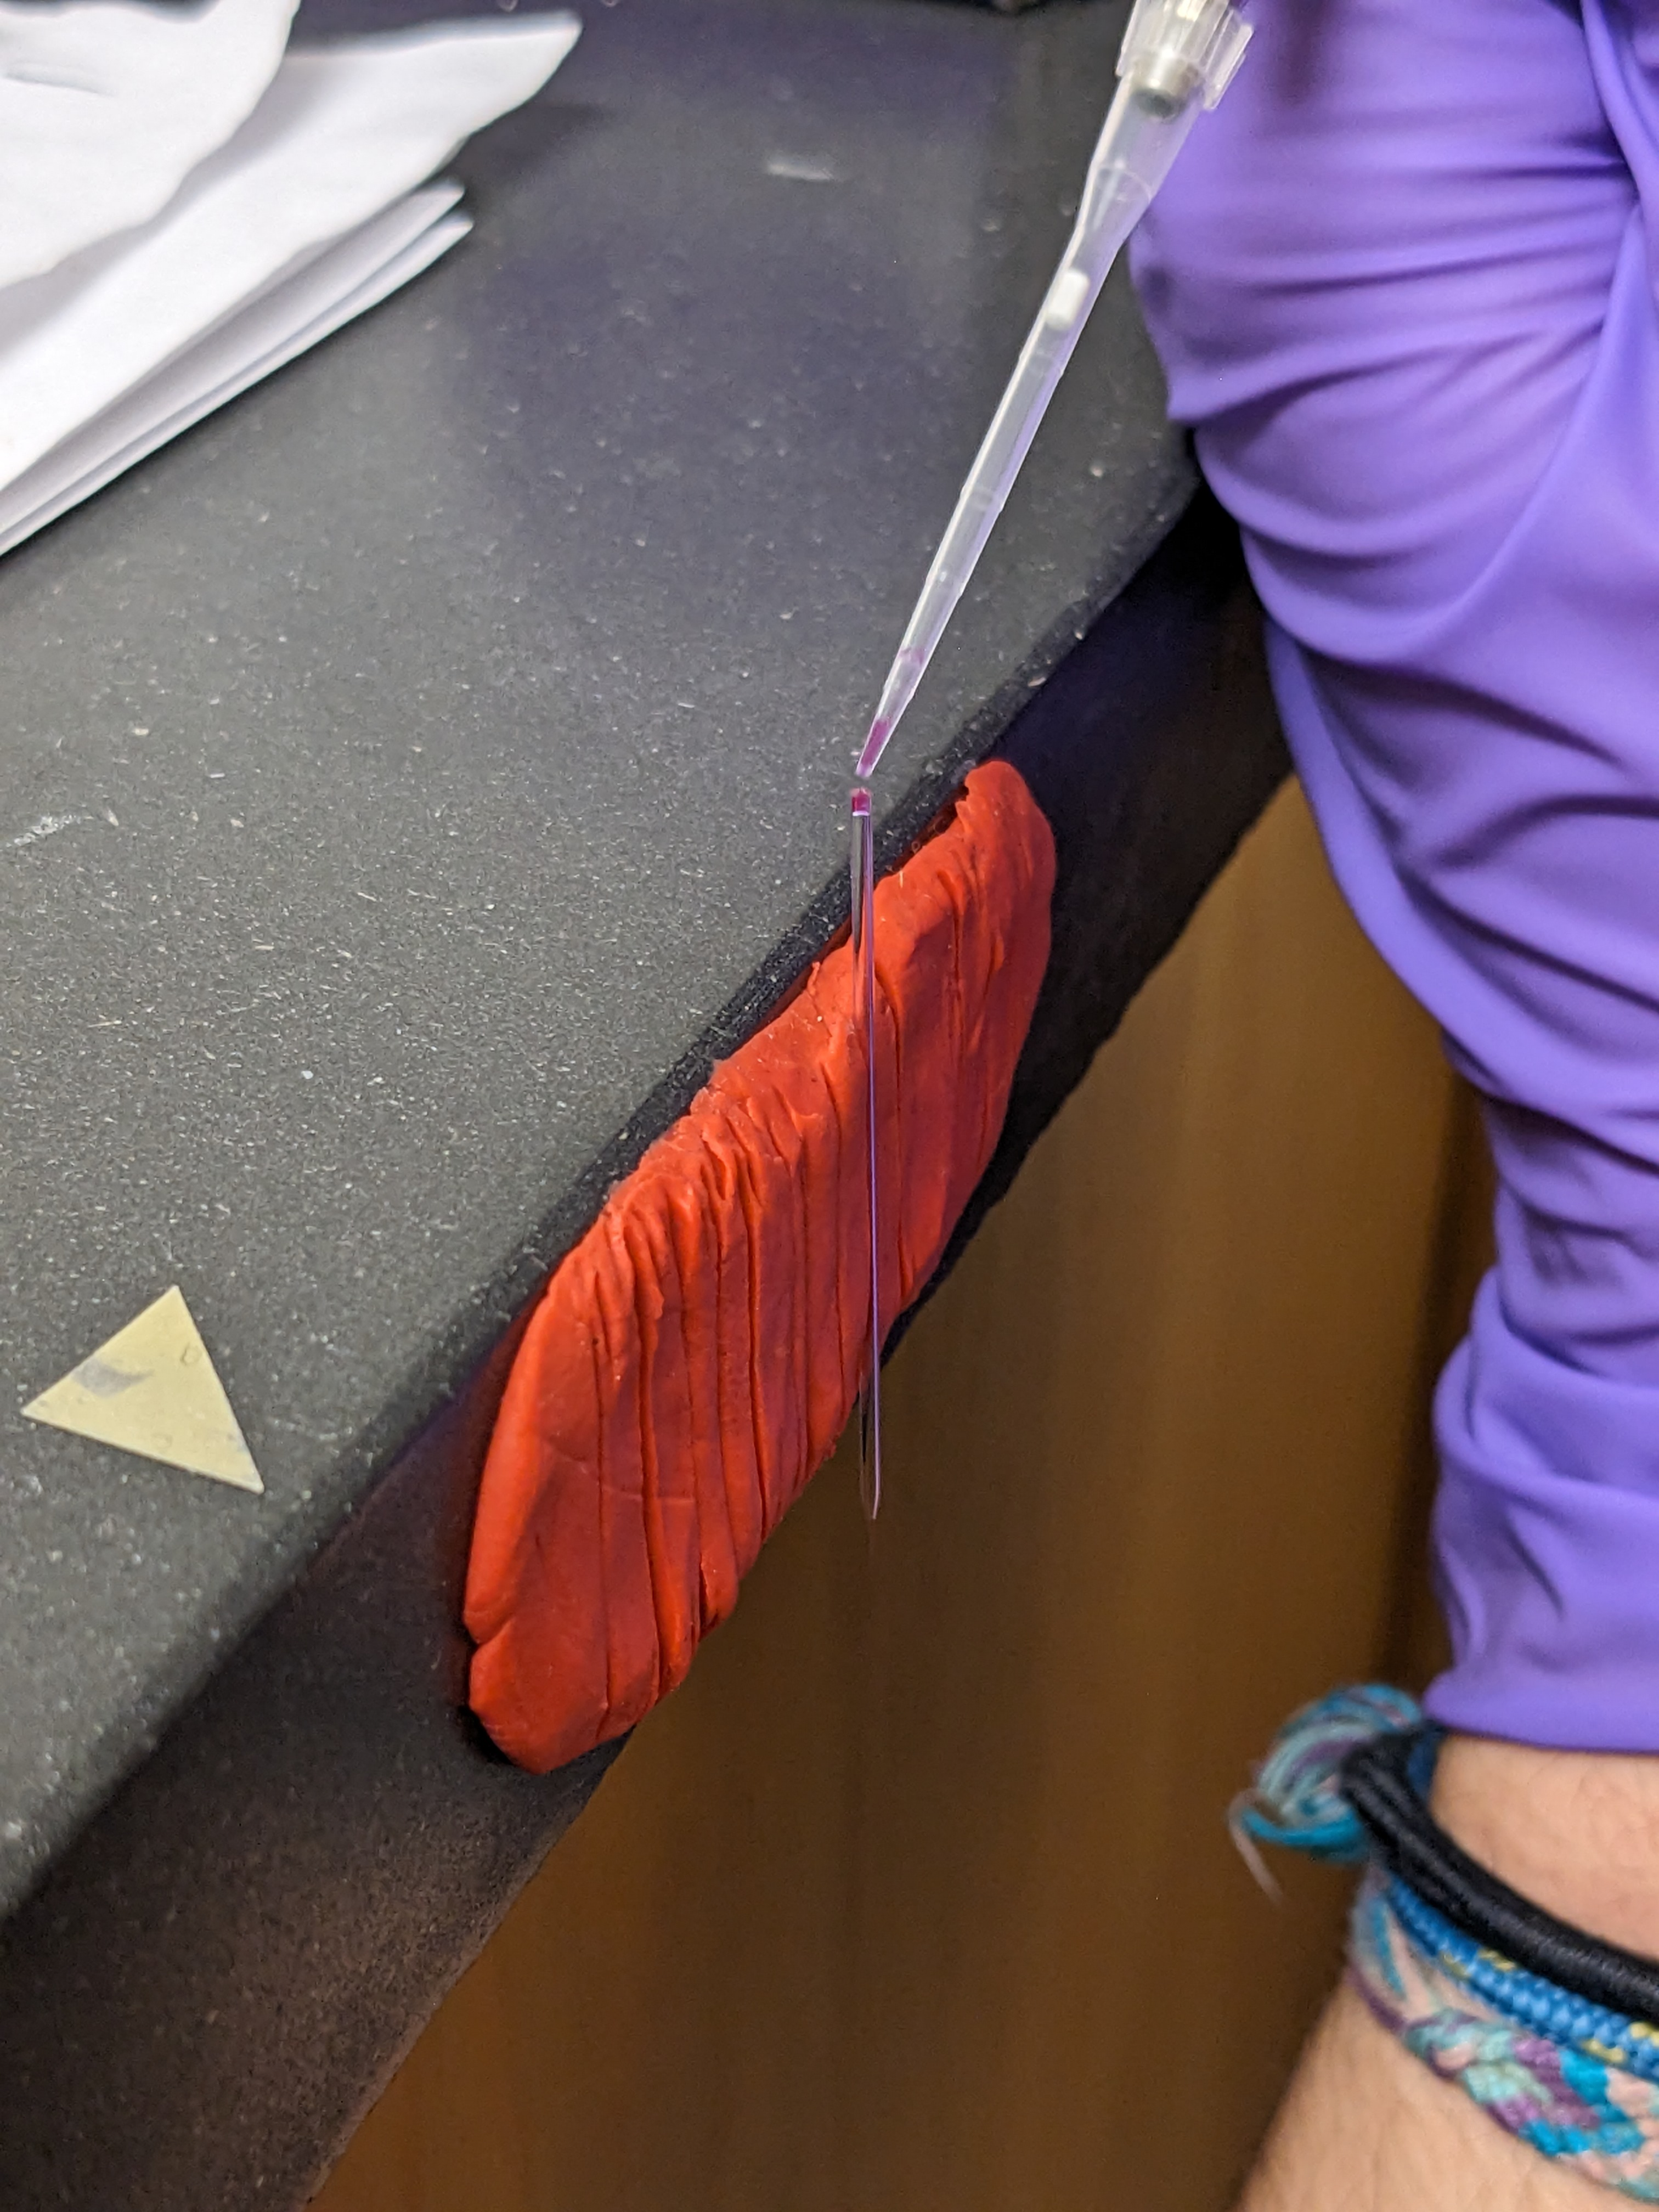
\includegraphics[width=3.125in,height=\textheight]{micro_photos/included/needle_filling.jpg}

}

\caption{Filling needles}

\end{figure}

Mount needle onto the macromanipulator:

\begin{figure}

\begin{minipage}[t]{0.50\linewidth}

{\centering 

\raisebox{-\height}{

\includegraphics{micro_photos/included/needle_holder1.jpg}

}

}

\subcaption{\label{fig-holder1}Insert needle into needle holder, end
first, make sure needle end is visible}
\end{minipage}%
%
\begin{minipage}[t]{0.50\linewidth}

{\centering 

\raisebox{-\height}{

\includegraphics{micro_photos/included/needle_holder2.jpg}

}

}

\subcaption{\label{fig-holder2}Needle in needle holder}
\end{minipage}%

\caption{\label{fig-eggs}Using the needle holder (aka grip head)}

\end{figure}

\begin{figure}

\begin{minipage}[t]{0.50\linewidth}

{\centering 

\raisebox{-\height}{

\includegraphics{micro_photos/included/macromanipulator.jpg}

}

}

\subcaption{\label{fig-macroman}Take off capillary holder (metal rod)
and screw in needle holder}
\end{minipage}%
%
\begin{minipage}[t]{0.50\linewidth}

{\centering 

\raisebox{-\height}{

\includegraphics{micro_photos/included/needle_holder3.jpg}

}

}

\subcaption{\label{fig-holder3}Make sure that the capillary holder is at
30°}
\end{minipage}%

\caption{\label{fig-eggs}Setting up macromanipulator}

\end{figure}

\hypertarget{the-microinjection-setup}{%
\subsection{The microinjection setup}\label{the-microinjection-setup}}

\begin{figure}

\begin{minipage}[t]{0.50\linewidth}

{\centering 

\raisebox{-\height}{

\includegraphics{micro_photos/included/confocal_microscope2.jpg}

}

}

\subcaption{\label{fig-macroman}}
\end{minipage}%
%
\begin{minipage}[t]{0.50\linewidth}

{\centering 

\raisebox{-\height}{

\includegraphics{micro_photos/included/confocal_microscope.jpg}

}

}

\subcaption{\label{fig-holder3}}
\end{minipage}%

\caption{\label{fig-eggs}Confocal microscope set up}

\end{figure}

\hypertarget{preparing-sea-water}{%
\subsection{Preparing sea water}\label{preparing-sea-water}}

For embryonic development:

Prepare a beaker (1000 ml) with sea water (12°C, RO + instant ocean
salt). Check for correct salinity (\textasciitilde33\%)! Adjust salinity
if needed. Place in 15°C fridge.

For during the microinjection:

Pour 25 ml of the filtered sea water into a 50 ml centrifuge tube and
add 25ul of 1M 3-aminotriazole (3-AT) stock solution\footnote{3-AT stock
  soluion: Prepare 1 M stock solution of 3-aminotriazole (3-AT, MW =
  84.08) by dissolving 0.84 g of 3-AT in 10 ml of ddH2O. This solution
  can be stored at 4 °C for up to 6 months.} to it. ``Label as 3AT
filtered sea water''. Place the 3AT sea water on ice.

\hypertarget{preparing-the-petri-dish}{%
\subsection{Preparing the petri dish}\label{preparing-the-petri-dish}}

Take a PS-coated petri dish\footnote{PS coated dishes: Prepare 1\%
  solution of protamine sulfate (PS) by adding 0.5 g of PS to 50 ml of
  deionized, distilled water (ddH2O) in a 50 ml conical tube. Shake well
  at high speed on a bench shaker at room temperature for 1-2 hr to
  ensure complete dissolution of PS. This solution can be stored at 4 °C
  for at least 3 months (make sure to completely dissolve gel-like
  precipitate before each use). Take a sleeve of 60 mm x 15 mm
  polystyrene Petri dishes and lay out both lids and bottoms on the
  bench. Warm up PS solution to room temperature. Pour 1\% PS solution
  in each dish (both bottoms and lids can be used) just enough to cover
  the surface, leave for at least 2 min. The leftover PS solution can be
  reused many times within 3 months when stored at 4°C. Place PS-treated
  dishes in a beaker filled with distilled water (dH2O). Leave the
  beaker under running dH2O for at least 10 min. PS-coated dishes can be
  used immediately or air dry for storage. Cover them to prevent dust
  accumulation. They can be stored at room temperature for 1 month.},
mark middle with a straight black line with marker on the outer side of
the dish. Take a razor blade and make a cut parallel to the black line
halfway between the black line and the edge of the dish on the inner
side of the dish. This scratch will be important to break the injection
needle to adjust the flow of solution as needed.

\begin{figure}

{\centering \includegraphics[width=3.125in,height=\textheight]{micro_photos/included/petri_dish_prep.jpg}

}

\caption{Prepared petri dish}

\end{figure}

Pipette 4 ml of 1 mM 3-AT sea water (prepared in the first step of
``Collecting eggs and sperm'') into the PS-coated dish using a transfer
pipette.

Place petri dish under microscope, such that the scratch mark is on the
left.

Switch on the microscope and the FemtoJet 4i. Make sure to detach the
injection tube first!

\begin{figure}

\begin{minipage}[t]{0.33\linewidth}

{\centering 

\raisebox{-\height}{

\includegraphics{micro_photos/included/microscope_ON_button.jpg}

}

}

\subcaption{\label{fig-microON}Switch on power strip to switch on
microscope}
\end{minipage}%
%
\begin{minipage}[t]{0.33\linewidth}

{\centering 

\raisebox{-\height}{

\includegraphics{micro_photos/included/microinjector_ON_button.jpg}

}

}

\subcaption{\label{fig-microinjON}Switch on FemtoJet with the button on
the back}
\end{minipage}%
%
\begin{minipage}[t]{0.33\linewidth}

{\centering 

\raisebox{-\height}{

\includegraphics{micro_photos/included/microinjector_build_pressure.jpg}

}

}

\subcaption{\label{fig-microinjBUILD}FemtoJet starts to build up
pressure automatically, make sure tube is disconnected}
\end{minipage}%

\caption{\label{fig-eggs}Turning on equipment}

\end{figure}

Once the pressure has built up, attach the injection tube to the
FemtoJet (TODO note about the ring size). If you see the error message
below, make sure that the injection tube is correctly attached to the
FemtoJet, and that the needle in the needle holder is all the way in and
the tube is screwed on right.

\begin{figure}

{\centering \includegraphics[width=3.125in,height=\textheight]{micro_photos/included/microinjector_error.jpg}

}

\caption{Microinjector error}

\end{figure}

Default microinjector settings: Manual, 120, 40.

Lower needle into the sea water using the macromanipulator. Once the
needle touches the water, find the needle through the microscope and
lower/adjust focus until the needle touches the bottom of the petri
dish. Navigate to the scratch mark. Gently touch the scratch with the
end of the needle to break it very slightly. Check with the fluorescent
light that there is a good flow of solution.

\begin{figure}

\begin{minipage}[t]{0.25\linewidth}

{\centering 

\raisebox{-\height}{

\includegraphics{micro_photos/included/breaking_needle.jpg}

}

}

\subcaption{\label{fig-break}Broken needle with scratch mark}
\end{minipage}%
%
\begin{minipage}[t]{0.38\linewidth}

{\centering 

\raisebox{-\height}{

\includegraphics{micro_photos/included/speed_liquid_from_needle.mp4}

}

}

\subcaption{\label{fig-speed1}High speed of injection solution flow,
this will be hard to work with}
\end{minipage}%
%
\begin{minipage}[t]{0.38\linewidth}

{\centering 

\raisebox{-\height}{

\includegraphics{micro_photos/included/speed_liquid2.mp4}

}

}

\subcaption{\label{fig-speed2}Ideal speed of injection solution flow}
\end{minipage}%

\caption{\label{fig-eggs}Setting up needle in the sea water}

\end{figure}

\hypertarget{rowing-the-eggs-and-fertilization}{%
\subsection{Rowing the eggs and
fertilization}\label{rowing-the-eggs-and-fertilization}}

Lift the needle out of the liquid using the macromanipulator to avoid
breaking the needle during rowing of the eggs.

Row 10ul of dejellied eggs in a straight line using a 10 ul pipette tip.
If the eggs have been sitting in the glass beaker for a while, they tend
to stick to the bottom and pipetting up with the 10ul pipette tip might
become difficult. Use a 3ml transfer pipette to pipette up and down near
the eggs to stir them up.

\begin{figure}

{\centering 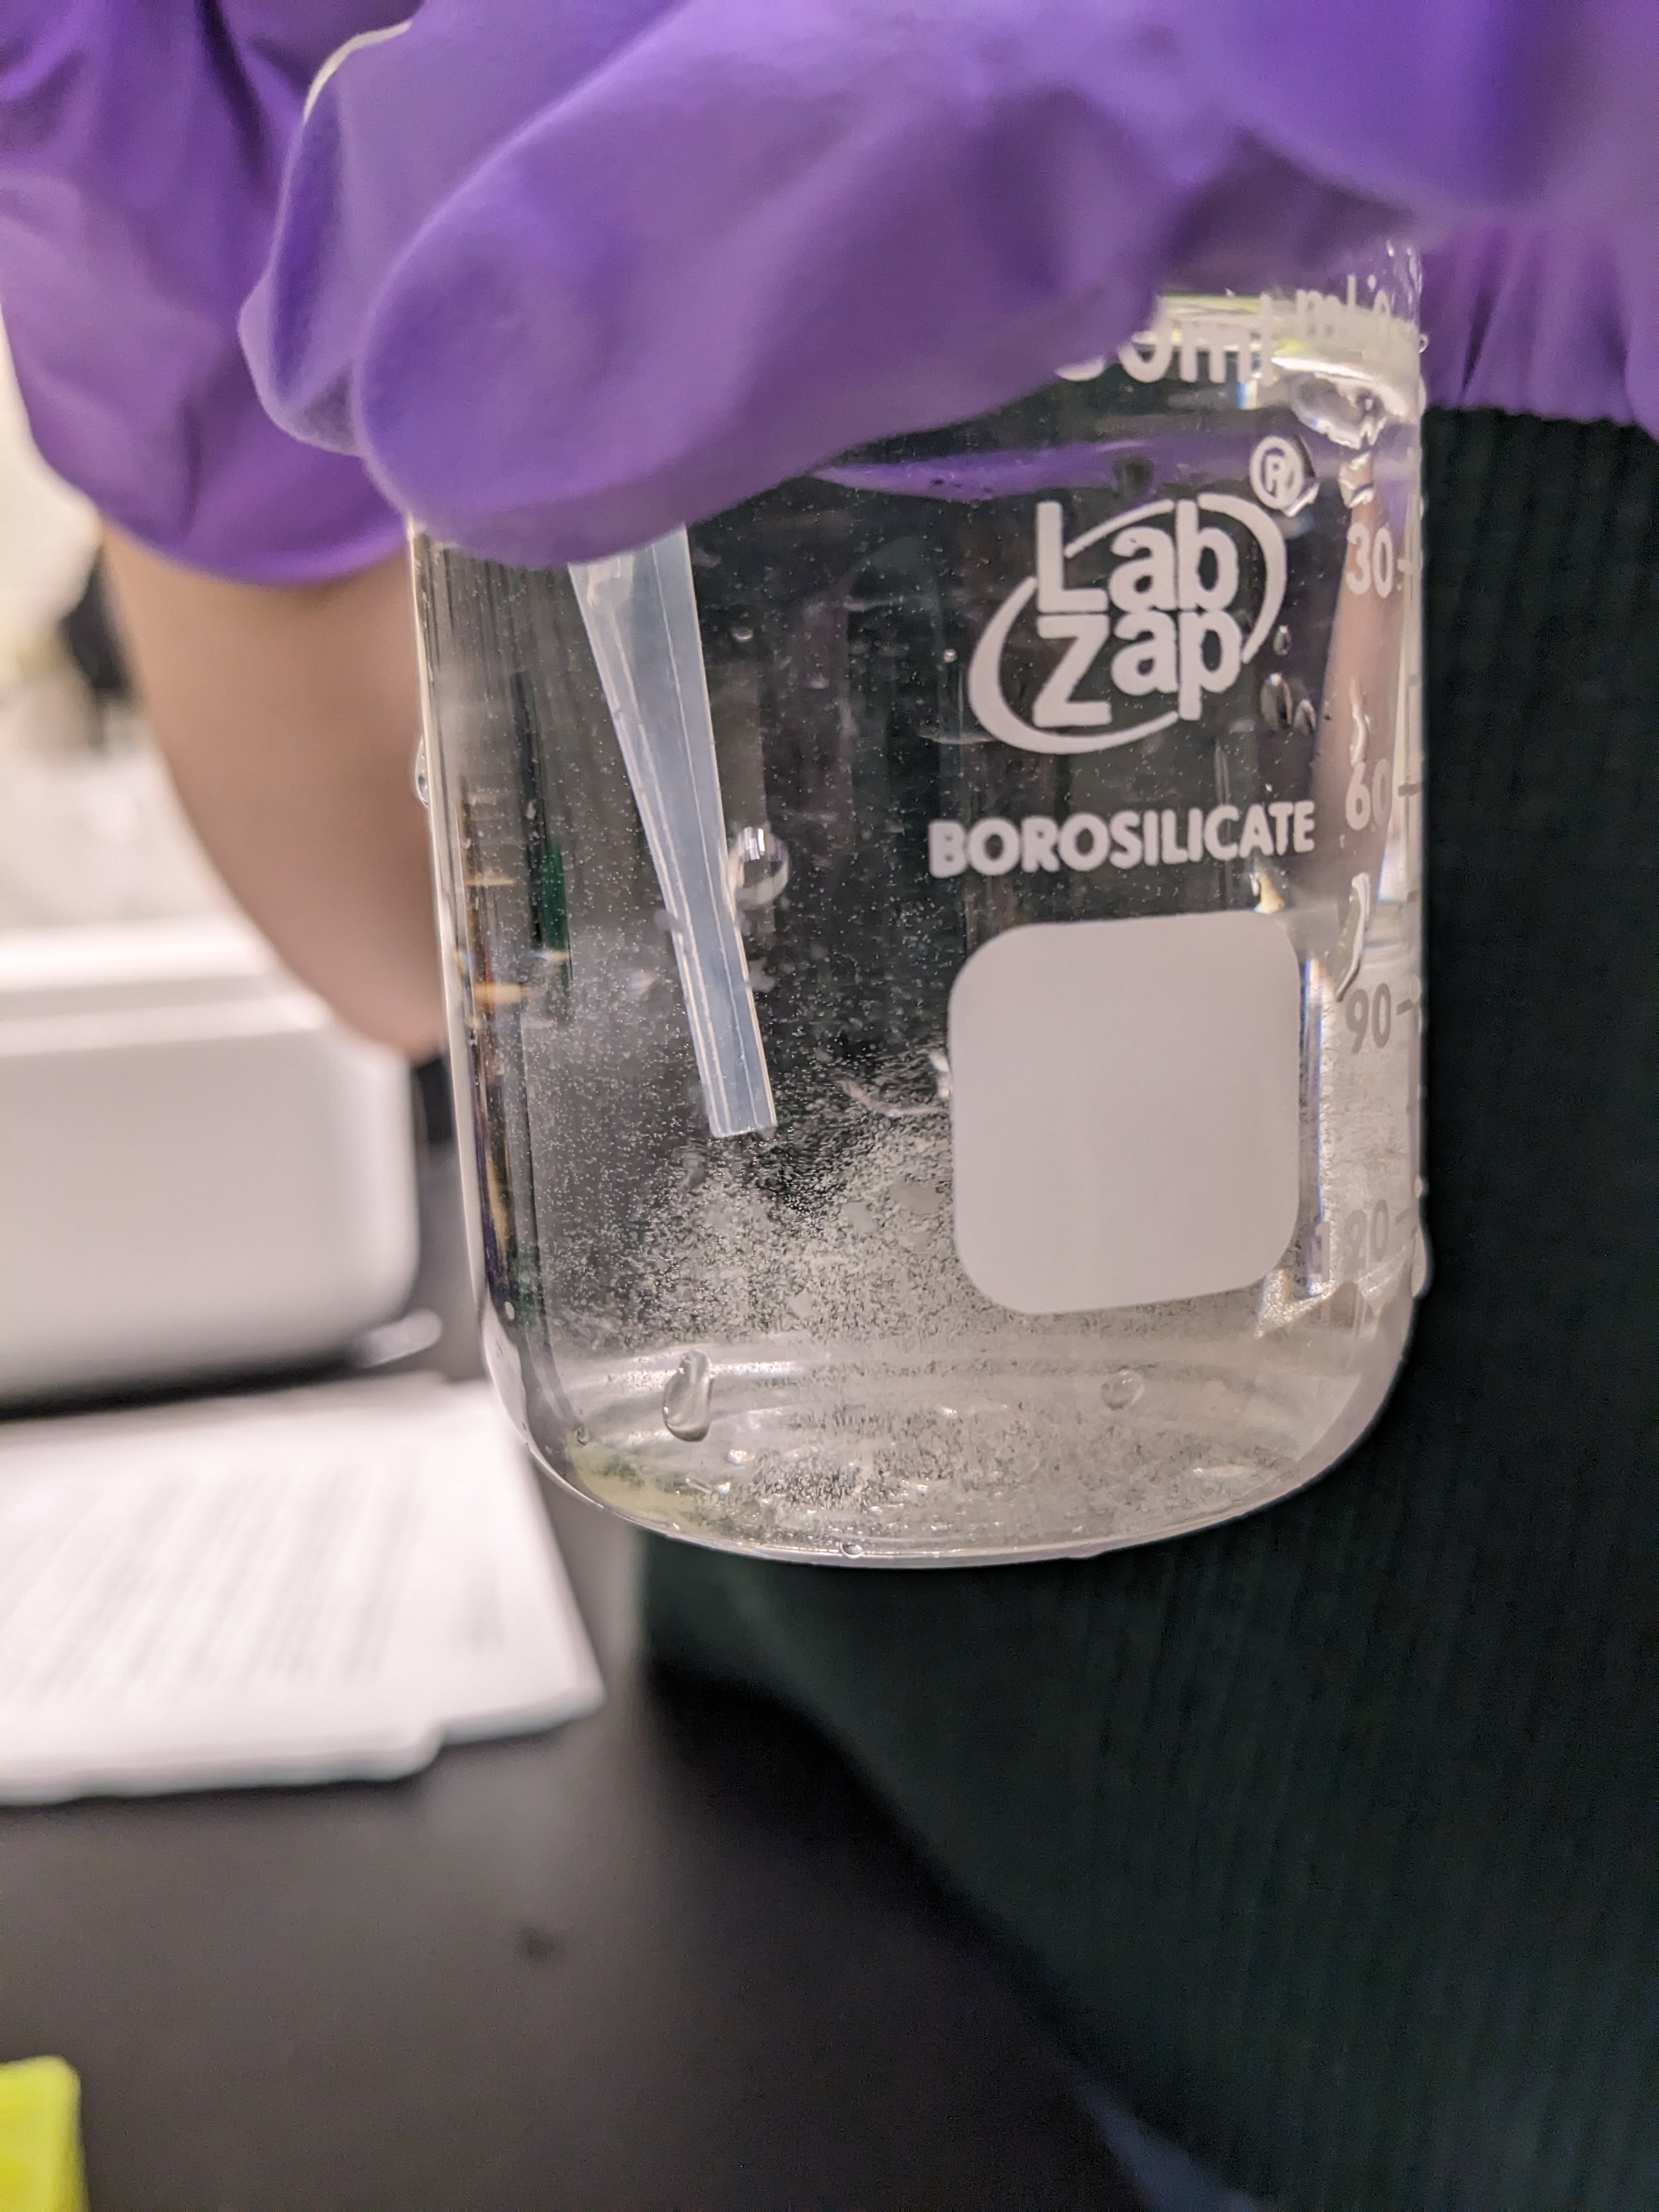
\includegraphics[width=3.125in,height=\textheight]{micro_photos/included/stir_eggs.jpg}

}

\caption{Stir eggs with transfer pipette}

\end{figure}

Row the eggs on the petri dish parallel and in-between the two lines
mentioned above (marker and scratch mark lines) using a pipette. Row the
eggs right before the injections, because fertilization problems may
occur due to prolonged exposure to 3-AT sea water. Gently press the tip
of the pipette to the bottom of the petri dish on the top, and move down
in a line while continuously pushing out the eggs from the pipette tip.

\begin{figure}

{\centering \includegraphics[width=6.25in,height=\textheight]{micro_photos/included/rowing.jpg}

}

\caption{Row eggs in the petri dish}

\end{figure}

Find the eggs with the microscope. Lower the needle back into the sea
water and gently poke an egg to make sure they are stuck to the bottom.

Dilute and activate the sperm by adding 1ul of sperm into 100ul of sea
water and mixing the water with the pipette tip for a few minutes until
there are no chunks left and the solution is opaque and homogeneous. Add
10ul of diluted sperm directly on top of the top eggs. Submerge the tip
and expel the sperm directly above, but be careful not to touch the
eggs. Only fertilize a portion of the eggs at a time since the
fertilized eggs become hardened and impossible to inject 10-15 minutes
after fertilization. Once the fertilized eggs are injected and you move
down to unfertilized eggs, repeat this step including the dilution of
the sperm as after 10-15 minutes the activated sperm become less
fertile.

\begin{figure}

{\centering \includegraphics[width=6.25in,height=\textheight]{micro_photos/included/fertilized.jpg}

}

\caption{Fertilized eggs with fertilization envelop}

\end{figure}

\hypertarget{microinjection-of-fertilized-eggs}{%
\subsection{Microinjection of fertilized
eggs}\label{microinjection-of-fertilized-eggs}}

Once the eggs are fertilized (the fertilization envelop appears), push
the needle against a fertilized egg such that it makes a dent in the
middle of the cell.

Hit the side of the microscope with your hand to make the needle enter
the cell. You might need to hit it repeatedly.

You can tell that the needle has entered the cell if:

\begin{enumerate}
\def\labelenumi{\alph{enumi})}
\item
  you see the tension of the cell wall is released and the dent created
  by the needle disappears
\item
  you see some movement inside the cell as the flow of the injection
  solution from the needle in disturbing the cellular content
\end{enumerate}

After pressing the pedal, you should see a light area appear around the
needle - this is called the injection bolus. Once the size for the
injection bolus reaches 1/4 of the volume of the cell, pull out the
needle. The cell should remain intact without anything flowing out of
it. The injection bolus should disappear after 30 sec - 1 min.

Move to the next cell using the micromanipulator and the stage
controller. Repeat.

\begin{figure}

{\centering \includegraphics[width=6.25in,height=\textheight]{micro_photos/included/microinjection_example.mp4}

}

\caption{Microinjection of fertilized eggs. Note: in this video the
injection bolus didn't reach the appropiate 1/4 size.}

\end{figure}

When done (fertilized eggs hardened or injected enough eggs), remove the
dish from the stage and carefully aspirate out water using a transfer
pipette.

Do not let the zygotes dry. Quickly add fresh prechilled sea water (from
the 15°C fridge) to cover the dish. Label the petri dish (your name,
date, time in hours and minutes, number of eggs injected, type of
injection solution used). Incubate the embryos at 15°C.

\hypertarget{visualising-embryos}{%
\subsection{Visualising embryos}\label{visualising-embryos}}

WIP



\end{document}
